% Chapter 3

\chapter{System Architecture and Experimental Framework}
\label{ch:system_architecture}

This chapter presents the system architecture and experimental framework used throughout the thesis. The chapter describes the robotic platforms, sensing configuration, ROS~2 and Gazebo integration, control and coordination modules, mission scenario, and system-level information flow. The purpose of the chapter is to show how the individual technical components are assembled into one coherent UAV--UGV experimentation pipeline that supports both rule-based maneuver generation and learning-based trajectory evaluation.

\section{Overall System Overview}

The overall system is organized as a cooperative aerial-ground robotic framework operating in simulation. At the center of the framework is one UGV that serves as the primary maneuvering platform and two UAVs that serve as supporting scout agents. The UGV is responsible for goal-directed movement, obstacle response, and eventual mission completion. The UAVs provide a broader spatial perspective and maintain scout positions relative to the UGV, thereby supplying cooperative context during navigation. This general architectural direction is consistent with the broader value of heterogeneous UAV--UGV cooperation reported by \citeauthor{asadi2020integrated} \citep{asadi2020integrated}.

The experimental framework is implemented in the Baylands simulation world and uses ROS~2 as the middleware layer for perception, control, logging, and inter-module communication. \citeauthor{gazeboros2docs} provide the physics-based simulation environment and interaction workflow used through Gazebo \citep{gazeboros2docs}. A ROS--Gazebo bridge is used to expose simulated sensor data and model states as ROS~2 topics, allowing the same middleware workflow to be used for control logic, data recording, and later learning-based evaluation, consistent with the integration described by \citeauthor{rosgzbridgedocs} \citep{rosgzbridgedocs}.

\begin{figure}[tbp]
    \centering
    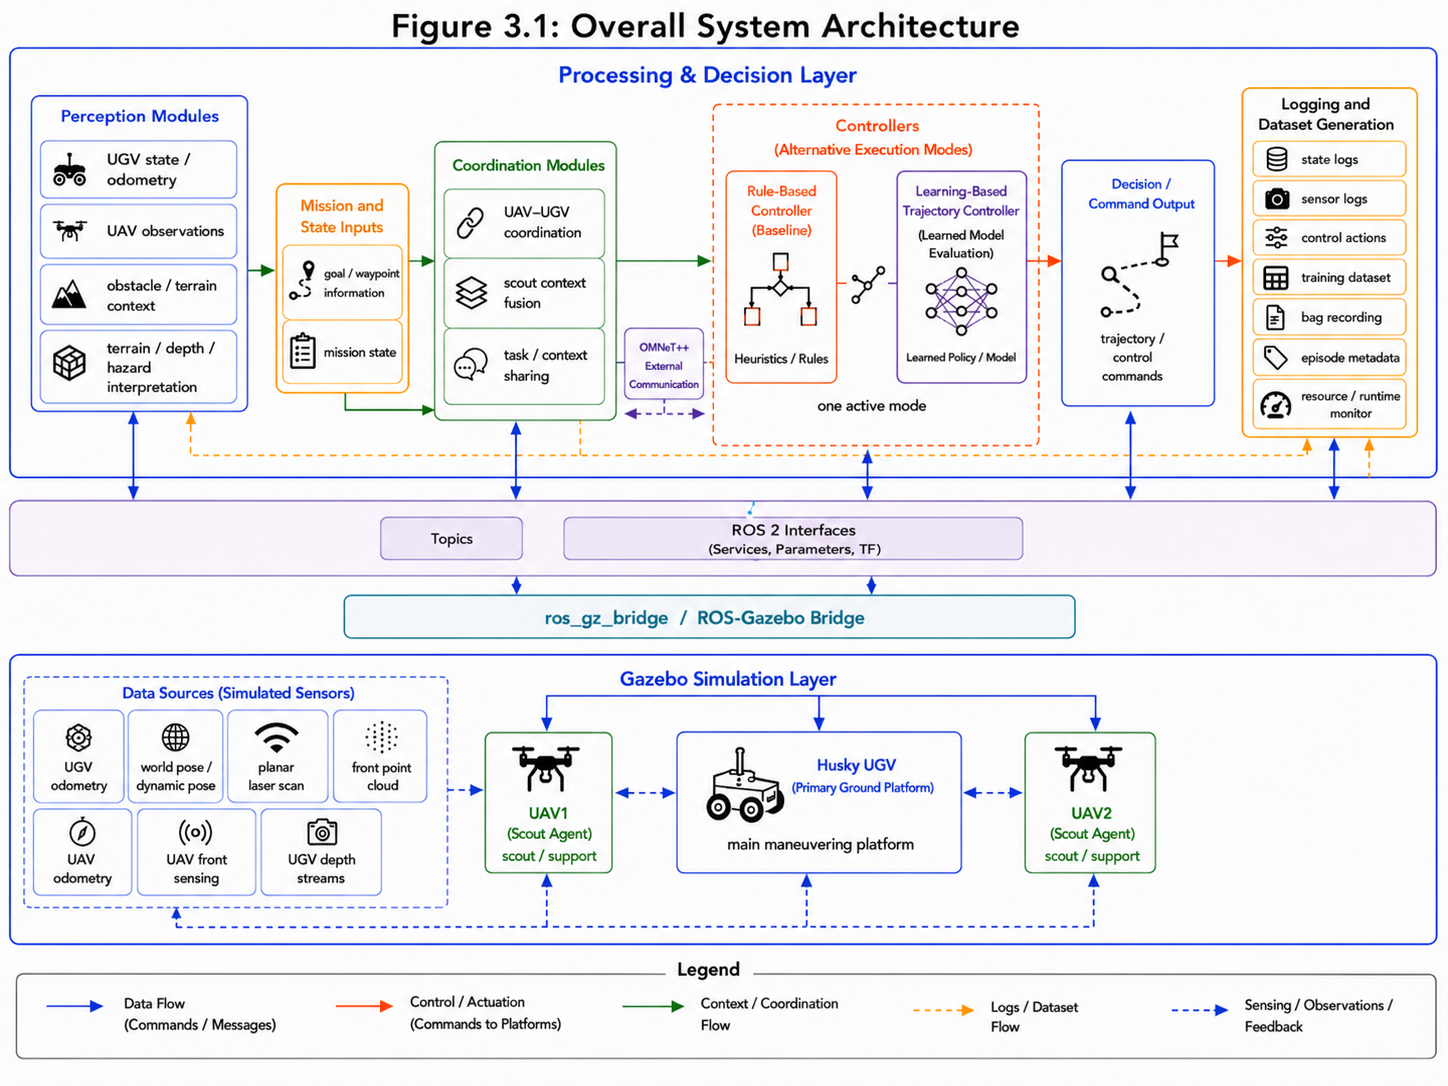
\includegraphics[width=\textwidth]{./gfx/image_3_1.png}
    \caption{Overall system architecture of the cooperative UAV--UGV navigation framework. The figure illustrates the Gazebo simulation layer, the ROS~2 middleware and interface layer, the ROS--Gazebo bridge, perception and coordination modules, alternative rule-based and learning-based UGV control modes, OMNeT++-supported communication, and the logging and dataset-generation components used throughout the thesis.}
    \label{fig:overall_system_architecture}
\end{figure}

Figure~\ref{fig:overall_system_architecture} presents the complete architecture of the proposed cooperative UAV--UGV framework. The system is structured into a Gazebo simulation layer, a ROS~2 communication and interface layer, and a processing and decision layer. The figure also shows the two alternative UGV control modes used in the thesis, namely the rule-based baseline controller and the learning-based trajectory controller, together with the supporting UAV scout agents, the OMNeT++ communication component, and the data-recording pipeline that supports later training and evaluation.

The architecture supports two closely related execution flows. The first flow is the rule-based baseline, where the UGV uses explicit maneuver logic and the UAVs operate as coordinated scout agents. The second flow is the learning-based evaluation stack, where trained trajectory-model weights are reinserted into the live simulation so that learned trajectory prediction can replace the rule-based maneuver generator while the rest of the system-level infrastructure remains available. This shared architecture is important because it allows the learned-controller experiments to be compared against the rule-based baseline under nearly identical environmental and middleware conditions.

\section{UGV Platform Description}

The ground platform used in the thesis is a Husky-based mobile robot instantiated from the Marble Husky sensor configuration model provided through the Open Robotics model repository \citeauthor{openrobotics2023husky} \citep{openrobotics2023husky}. Within the experimental setup, the Husky functions as the main navigation agent and is the only platform that is directly evaluated for goal-reaching performance. The UGV receives motion commands through velocity-based control and continuously publishes odometry and state information through the ROS~2 communication layer. In practical terms, this makes the UGV the main execution platform in both the rule-based and learning-based experiments.

\begin{table}[tbp]
    \caption{Summary of the UGV platform used in the thesis.}
    \label{tab:ugv_platform_summary}
    \centering
    % Column widths: c1 = 0.24\textwidth, c2 = remaining width (X)
    \begin{tabularx}{\textwidth}{@{}>{\raggedright\arraybackslash}p{0.24\textwidth}X@{}}
        \toprule
        \textbf{Attribute} & \textbf{Description} \\
        \midrule
        Platform & Husky UGV based on the Marble Husky Sensor Config 1 model. \\
        Primary role & Main ground maneuvering platform and the only agent directly evaluated for goal-reaching performance. \\
        Control interface & Velocity-based control through ROS~2 command topics. \\
        Main state outputs & Odometry, controller state, executed motion, and world-referenced pose context. \\
        Cooperative role & Spatial anchor for UAV scout formation and the main receiver of cooperative support context. \\
        Role in learning pipeline & Source of trajectory-training samples during data generation and target platform for learned-controller redeployment. \\
        \bottomrule
    \end{tabularx}
\end{table}

Table~\ref{tab:ugv_platform_summary} summarizes the core characteristics of the UGV platform in relation to the operational and learning-based goals of the thesis.

Architecturally, the UGV fulfills three closely related roles. First, it is the primary maneuvering platform because all final motion commands are applied to it. Second, it is the main point of local terrain and obstacle interaction because its sensing is positioned closest to the driving surface and therefore captures the immediate navigational consequences of uneven terrain, nearby objects, and path constraints. Third, it is the spatial anchor around which the UAV scout formation is organized. This means that the UGV is not only the main subject of navigation, but also the reference platform for cooperative aerial-ground coordination.

The UGV is equally central to the learning pipeline developed in the thesis. During rule-based operation, its states, controller outputs, and contextual signals are recorded and later transformed into structured trajectory-learning samples. During learned-controller evaluation, the trained model consumes recent UGV history together with compact local and relational features in order to predict a short-horizon future trajectory for this same platform. The Husky therefore serves as the common operational link between simulation, data generation, model training, and live model redeployment.

This choice of platform is appropriate for the thesis because it supports a clear separation between local ground interaction and aerial support. The Husky remains responsible for actual maneuver execution and goal progression, while the UAVs contribute supporting context rather than replacing the ground vehicle's role. As a result, the UGV platform provides a stable and interpretable basis for comparing handcrafted maneuver logic against learned short-horizon trajectory prediction under the same cooperative mission structure.

\section{UAV Platform Description}

The aerial component of the framework consists of two UAVs instantiated from the CERBERUS M100 sensor configuration model available through Open Robotics \citeauthor{openrobotics2023m100} \citep{openrobotics2023m100}. These two UAVs are used symmetrically as scout agents. Rather than acting as independent mission vehicles, they are assigned support roles relative to the UGV and are configured to maintain scout slots around it during navigation. In practical terms, this means that the UAVs are responsible for providing cooperative aerial context while the UGV remains the main ground maneuvering platform.

\begin{table}[tbp]
    \caption{Summary of the UAV scout platforms used in the thesis.}
    \label{tab:uav_platform_summary}
    \centering
    % Column widths: c1 = 0.24\textwidth, c2 = remaining width (X)
    \begin{tabularx}{\textwidth}{@{}>{\raggedright\arraybackslash}p{0.24\textwidth}X@{}}
        \toprule
        \textbf{Attribute} & \textbf{Description} \\
        \midrule
        Platform & Two UAV scout agents based on the CERBERUS M100 sensor configuration model. \\
        Quantity and arrangement & Two aerial agents deployed symmetrically around the UGV, with one left-support scout and one right-support scout. \\
        Primary role & Cooperative aerial support for the UGV rather than independent goal execution. \\
        Main behaviors & Slot following, elevated scout positioning, return-to-UGV behavior, and goal-oriented landing at mission completion. \\
        Main state outputs & Odometry, controller state, and scout-report information used for coordination and evaluation. \\
        Role in learning pipeline & Source of relational context through UAV position, motion, and support geometry relative to the UGV. \\
        \bottomrule
    \end{tabularx}
\end{table}

Table~\ref{tab:uav_platform_summary} summarizes the key characteristics of the UAV scout platforms in relation to their cooperative role in the thesis framework.

In the implemented setup, the UAVs are designed to follow the UGV while holding elevated scout positions ahead of it at a high operating altitude. Their placement is intentionally asymmetric in sign but symmetric in role: one UAV occupies a left-support slot and the other occupies a right-support slot. This arrangement is intended to provide spatially distributed support around the UGV while still preserving a simple and interpretable coordination geometry. The UAVs also include return-to-UGV and landing behaviors so that they can remain operationally coupled to the ground mission rather than acting as isolated observers.

Architecturally, the UAVs contribute in two distinct ways. In the rule-based system, they contribute terrain-related and obstacle-related support through scouting logic, readiness signals, and state reporting. In the learning-based framework, they provide relational context through their relative positions and motion states. This makes the UAVs important even when the learned model is not directly consuming high-level symbolic scout semantics. Their presence changes the geometry of the cooperative system, and that geometry becomes part of both the rule-based and learning-based evaluation flows.

This aerial-ground division of labor is important for the thesis design. The UAVs extend the spatial awareness of the overall system, but they do not replace the UGV's role as the primary decision executor. Instead, they act as structured support agents whose behavior improves coordination, enriches contextual information, and makes the navigation problem meaningfully multi-agent without shifting final maneuver authority away from the ground platform.

\section{Sensor Configuration and Data Sources}

The overall framework relies on a mixture of state, proximity, depth-related, and derived coordination signals. For the UGV, the most important raw data sources are odometry, world-frame pose updates, planar laser scan measurements, front-facing point-cloud information, and UGV-side depth-image streams exposed through the ROS--Gazebo bridge. In the rule-based stack, these depth-image channels support optional depth-based terrain or scene interpretation in addition to local obstacle reasoning, state tracking, and dataset export. This combination of state and scene-level sensing is consistent with the broader trend toward richer terrain interpretation for ground vehicles discussed by \citeauthor{chen2021cnn} \citep{chen2021cnn}.

The UAVs provide their own odometry streams together with forward obstacle-sensing channels used for local awareness and scout safety. In the implemented setup, the UAVs are not treated as primary RGB-D data sources in the same way as the UGV-side depth pipeline. Instead, they contribute mobile support context through position, motion, local obstacle status, and scout reporting. This distinction is important because the architecture exposes more raw sensing channels than are ultimately consumed in every experimental stage.

\begin{table}[tbp]
    \caption{Main sensor and data sources used in the cooperative UAV--UGV framework.}
    \label{tab:sensor_data_summary}
    \centering
    \small
    \setlength{\tabcolsep}{4pt}
    \renewcommand{\arraystretch}{1.15}
    % Column widths: c1 = 0.18\textwidth, c2 = 0.22\textwidth, c3 = remaining width (X)
    \begin{tabularx}{\textwidth}{@{}>{\raggedright\arraybackslash}p{0.18\textwidth}>{\raggedright\arraybackslash}p{0.22\textwidth}X@{}}
        \toprule
        \textbf{Platform / source} & \textbf{Data type} & \textbf{Main purpose in the thesis} \\
        \midrule
        UGV & Odometry & Ego-state tracking, trajectory supervision, controller feedback, and learned-model history input. \\
        UGV & World pose / dynamic pose & Shared world-frame state reference for goal progress, logging, and multi-agent alignment. \\
        UGV & Planar laser scan & Local obstacle detection and clearance reasoning in both rule-based and learned-controller execution. \\
        UGV & Front point cloud & Forward obstacle geometry and local safety interpretation. \\
        UGV & Depth-image stream & Optional rule-based depth classification for terrain or scene interpretation. \\
        UAVs & Odometry & Relative motion context, scout-state tracking, and graph-style relational information for learning. \\
        UAVs & Front obstacle sensing & Local UAV safety, scout obstacle awareness, and support behavior regulation. \\
        Internal system signals & Controller states, scout reports, obstacle-clearance summaries, episode metadata, and resource logs & Coordination, evaluation, bag recording, dataset construction, and runtime comparison. \\
        \bottomrule
    \end{tabularx}
\end{table}

Table~\ref{tab:sensor_data_summary} summarizes the main sensor and internal data streams used throughout the thesis. A key design decision is that the final learning dataset does not rely on raw image tensors as direct training inputs. Instead, the exported training samples use compact state, clearance, goal, and relational features derived from the operational simulation. This makes the training representation lighter, more structured, and easier to connect back to the live control stack.

In addition to raw or bridged sensor streams, the system also produces higher-level internal data products. These include controller-state messages, scout reports, obstacle-clearance summaries, episode metadata, resource-usage logs, and recorded ROS bags. Such data products are especially important because they connect online execution with later learning. They make it possible to convert live multi-robot behavior into structured training samples and to compare rule-based and learned-controller execution using the same monitoring framework.

\section{ROS 2 and Gazebo Integration}

The system uses ROS~2 as its runtime middleware and Gazebo as its main simulation environment, following the interaction model documented by \citeauthor{gazeboros2docs} \citep{gazeboros2docs}. This combination allows robot models, sensors, and controllers to be developed in a modular way while keeping the execution environment close to contemporary robotic software practice. ROS~2 provides the topic-based communication backbone, timer-driven node execution, message transport, and logging interfaces used by the perception, coordination, and control modules.

Gazebo is responsible for the simulated world, model spawning, sensor simulation, and dynamics execution. The bridge layer between Gazebo and ROS~2 is essential because it exposes simulation data as ROS topics that can be consumed by custom nodes, as described by \citeauthor{rosgzbridgedocs} \citep{rosgzbridgedocs}. In the present framework, this includes dynamic world pose information, odometry, laser scan data, point clouds, and camera-related streams. The bridge therefore serves as the operational boundary between the physics simulation and the robotic middleware layer, allowing the same robotic software workflow to interact with simulated platforms in a reproducible way.

This integration pattern is reused across both the rule-based and learning-based stacks. In the rule-based baseline, the bridge feeds the handcrafted perception and control nodes that generate the original maneuver data. In the learned-controller stack, the bridge feeds the live inference nodes that consume model weights and generate trajectory-driven commands. This reuse is methodologically important because it ensures that the learned-controller experiments are not evaluated in an artificial offline environment but within the same live simulation infrastructure used to generate the original behavior data. As a result, the framework preserves continuity between data generation, model training, and live deployment.

\section{Control, Perception, and Coordination Modules}

The framework is built from multiple ROS~2 modules that divide the system into perception, control, coordination, and monitoring responsibilities. On the perception side, local obstacle-detection modules interpret scan and point-cloud information to produce actionable clearance or obstacle estimates for both the ground vehicle and the UAV scouts. In the rule-based stack, an additional depth-classification component converts UGV-side depth imagery into compact scene-level terrain or block indications. These perception modules reduce raw sensor complexity and convert it into forms that are more directly useful for maneuver logic.

On the control side, the main UGV controller exists in two variants. The first is the rule-based UGV controller, which uses explicit decision logic for goal progression, obstacle handling, terrain-aware behavior, and recovery. In the rule-based pipeline, a decision-fusion stage can combine local obstacle information, hazard-style guidance, and optional depth classification before the final UGV action is selected. The second control path is the learned UGV controller, which consumes trained model predictions and converts them into executable motion commands while still operating within the same live simulation loop. This separation is architecturally important because it allows the study to compare handcrafted maneuver logic against learned trajectory generation without rebuilding the entire system around the learned model.

Coordination modules connect the UGV and UAV behaviors. The UAV scout driver maintains the aerial support formation, including takeoff, slot tracking, return-to-UGV behavior, and goal-oriented descent behavior. Additional coordination components handle scout readiness, scout reporting, and hazard-style aggregation so that the UGV can use cooperative context during execution. In the rule-based stack, this cooperative context can influence terrain confidence and maneuver prioritization through scout reports, scout summaries, and fused guidance signals. In the learning-based stack, UAV context is primarily represented through the relational features exported into the training and inference pipeline rather than through a separate symbolic decision map.

When communication-aware evaluation is enabled, additional bridge modules connect the robotics framework to the OMNeT++ layer. \citeauthor{varga2008omnet} describe OMNeT++ as a flexible event-based simulation environment for communication and network studies \citep{varga2008omnet}, which makes it suitable for communication-aware co-simulation in the present framework. A pose bridge exports selected live platform poses to the communication simulator, while a metrics bridge republishes communication-quality indicators back into ROS~2. This makes it possible for the learned-controller stack to remain connected to the same system architecture while also being evaluated under communication degradation.

The framework also includes supporting modules for episode metadata publication, run logging, bag recording, and runtime/resource monitoring. These components are not navigation controllers in the narrow sense, but they are central to the experimental framework because they create reproducible runs, enable later data extraction, and support the comparative evaluation strategy used in the thesis. Taken together, the module structure is intentionally layered: perception converts raw sensing into compact context, coordination shares aerial-ground information, control selects executable actions, and monitoring preserves each run for later analysis.

\section{Mission Scenario and Goal Definition}

All experiments are grounded in a common mission structure defined in the Baylands world. The mission consists of moving the UGV from a chosen spawn region toward a shared world-frame goal while coordinating the two UAV scouts around the ground platform. The same general world, shared-goal concept, and cooperative formation logic are reused across the rule-based and learning-based experiments so that the resulting behaviors remain comparable.

The UAVs are configured to climb to a dedicated scout altitude and maintain support slots relative to the UGV as the ground robot moves toward the goal. This creates a persistent aerial-ground geometry rather than a one-time information handoff. The mission therefore reflects continuous cooperative navigation rather than isolated waypoint exchange. Once the UGV reaches the goal, the UAVs transition from scout behavior toward goal-related landing behavior, thereby preserving a full mission lifecycle rather than ending the scenario as soon as the ground platform stops.

The scenario design is intentionally simple in its high-level objective but rich in its operational interactions. There is one primary maneuvering agent, two coordinated support agents, one shared goal, and multiple sensing and control layers operating simultaneously. This makes the scenario suitable for studying how local perception, cooperative context, and learning-based prediction interact in a unified setting. It also ensures that the same mission logic can support both trajectory-data generation and live redeployment of trained model weights.

\section{Information Flow Across the System}

The information flow across the system can be understood as a layered loop from sensing to decision to execution and back to logging. At the lowest level, Gazebo simulates the robots and their sensors. The ROS--Gazebo bridge then exposes these states and sensor streams to ROS~2. Perception modules consume the bridged data and produce simplified outputs such as obstacle clearances, depth-based terrain indications, or scout status messages.

These derived signals are then consumed by the control and coordination layers. In the rule-based configuration, the UGV controller combines local obstacle context, goal state, and UAV-related support information to select a maneuver. Where enabled, depth classification and fused guidance signals further refine the UGV-side decision path. In the learned-controller configuration, a trained trajectory model receives recent UGV history together with compact obstacle and UAV-context features and predicts a short future trajectory, which is then converted into executable commands by the live controller. In both cases, commands are sent back to the simulated UGV, closing the motion-control loop.

At the same time, the system records metadata about what occurred during execution. Odometry, controller states, scout reports, obstacle summaries, and related contextual information are logged and can be stored in ROS bags. These recordings are later transformed into episode frames and sliding-window training samples for the learning pipeline. When communication-aware evaluation is active, OMNeT++ metrics follow an additional path back into the ROS environment, where they can influence runtime confidence handling while still being recorded as part of the evaluation context.

The information flow therefore does not stop at online execution. It continues into the offline learning stage, where recorded behavior is converted into model-training data, and then returns again to live simulation when trained model weights are deployed back into the system. This closed experimental loop is one of the defining features of the framework. The system is not only a navigation simulator and not only a learning pipeline. It is an integrated architecture in which simulation, cooperative control, dataset generation, model training, live redeployment, and communication-aware evaluation are connected through a consistent set of data interfaces and execution assumptions.

Taken as a whole, Chapter~\ref{ch:system_architecture} establishes the technical foundation for the remainder of the thesis. The chapter has shown how the robotic platforms, sensing channels, middleware, control modules, mission setup, and information pathways are combined into one consistent experimental framework. On this basis, the next chapter can focus on the methodology itself, namely how the rule-based maneuver pipeline is designed, how the recorded data are transformed into learning samples, and how the resulting models are trained and evaluated within the same system.
